%% =============================================================================
%%  Manuscript for STATISTICS IN MEDICINE (John Wiley & Sons).
%%
%%  Typeset with Wiley's own authoring class, USG.cls, from WileyDesign.zip
%%  ("Optimal-Design-layout"). Wiley's LaTeX author guidelines are followed:
%%
%%    * USG.cls with the [AMA] reference-style option -- Statistics in
%%      Medicine cites in AMA style (numbered in order of appearance, Arabic
%%      SUPERSCRIPT numerals). The class loads NJDnatbib with [numbers,super]
%%      and issues \setcitestyle{super} for us, so plain \cite{} is correct.
%%    * One column. Wiley converts the manuscript to the journal's final
%%      specification at typesetting "regardless of the reference, font and
%%      column number format selected in the LaTeX manuscript".
%%    * Preamble kept minimal, as instructed. USG.cls already loads graphicx,
%%      booktabs, amsmath, amssymb, natbib, url, multirow, tabularx, dcolumn,
%%      float, rotating, subfig and hyperref, and defines its own caption
%%      format -- loading any of them again fights the class.
%%    * No custom fonts, no changed global spacing (\parindent, \parskip,
%%      \textwidth, \textheight), no new environments or macros.
%%    * Diacritics written as LaTeX codes (\'{a}, \~{n}) in references.bib.
%%
%%  SUPPORTING FILES REQUIRED TO COMPILE, all copied into this directory from
%%  WileyDesign/Optimal-Design-layout/:
%%    USG.cls  NJDnatbib.sty  NJDapacite.sty  LETTERSP.STY  mla.sty
%%    appendix.sty  algorithm.sty  algorithmicx.sty  wileyNJD-Chicago.bst
%%  plus WileyNJD-AMA.bst, which Wiley does not ship -- see the header of that
%%  file for what it is and how to replace it.
%%
%%  Compile:  pdflatex -> bibtex -> pdflatex -> pdflatex
%%  (Wiley suggest XeLaTeX; this class pulls Type1 STIX through the stix2
%%  package rather than fontspec, so pdflatex is sufficient and portable.)
%
%% =============================================================================
\documentclass[AMA]{USG}

% USG.cls draws its title-page furniture from an images/ folder and from two
% files in the working directory. All are copied from the template package.
% NOTE: the class hard-codes the sample journal's logo as allergy.eps. Ours is
% a BLANK EPS (the template's own empty.eps), so no other journal's branding
% appears on the title page. If the editorial office supplies the Statistics in
% Medicine masthead, drop it in as allergy.eps and delete images/allergy-eps-converted-to.pdf.
\graphicspath{{./}{./images/}}

% ---- FLOAT PLACEMENT -- one-line toggle ------------------------------------
% Floats sit inline, where they are declared, which is what Wiley's template
% does and what reads best for a reviewer.
%
% The journal's Author Guidelines ask for tables on separate pages after the
% reference list. That rule belongs to their traditional manuscript format;
% Statistics in Medicine offers Free Format submission ("submit your manuscript
% in the format of your choice, and Wiley will update the formatting for you
% into journal style if your manuscript is accepted"), so it costs nothing to
% ignore, and honoring it meant scattering "[Table 1 about here]" markers
% through the text.
%
% UNCOMMENT THE TWO LINES BELOW to defer every float to the end instead
% (tables first, one per page, with a marker at each point of first citation).
% If you do, note that USG.cls computes its "n of N" footer in an
% \AtEndDocument hook registered at class-load time, which runs BEFORE endfloat
% ships the deferred pages -- N then undercounts by exactly the number of float
% pages. The fix is to rewrite \LastPg from
% \AddToHook{enddocument/afterlastpage}; see notes for the exact block.
%\usepackage[tablesfirst,nolists]{endfloat}
%\renewcommand{\efloatseparator}{\clearpage}


\articletype{ORIGINAL ARTICLE}%

% The editorial office fills these in. Wiley's guidelines: "Authors can input
% these dates as '00' when the manuscript is being prepared."
\received{00 Month 0000}
\revised{00 Month 0000}
\accepted{00 Month 0000}

\journal{Statistics in Medicine}
\volume{00}
\copyyear{2026}
\startpage{1}
\articledoi{10.5281/zenodo.22089989}

\begin{document}

\title{Investigating Determinants of Birth Weight Using Bayesian Tree-Based
Nonparametric Modeling}

\author[1]{Adam M. Kurth}[https://orcid.org/0009-0001-8296-8108]
\author[2]{P. Richard Hahn}[https://orcid.org/0009-0009-8607-5671]

% Running heads. \titlemark doubles as the journal's "short title of up to 70
% characters"; the string below is 49 characters.
\authormark{KURTH \textsc{and} HAHN}
\titlemark{Dirichlet-Multinomial Trees for Birth Weight}

\address[1]{\orgdiv{Department of Biostatistics, }\orgname{Brown University
School of Public Health, }%
\orgaddress{\state{Providence, Rhode Island, }\country{USA}}}

\address[2]{\orgdiv{School of Mathematical \& Statistical Sciences,
}\orgname{Arizona State University, }%
\orgaddress{\state{Tempe, Arizona, }\country{USA}}}

% The journal asks for "the full address, including email, telephone and fax,
% of the author who is to check the proofs".
\corres{Adam M. Kurth, Department of Biostatistics, Brown University School of
Public Health, 121 South Main Street, Providence, RI 02903, USA.
(\email{adam\_kurth@brown.edu}) ~|~ Telephone: +1 (816) 289-1956 ~|~ Fax: none}

% Confirm before submitting: the journal asks for every sponsor and grant number.
\fundingInfo{This research received no specific grant from any funding agency
in the public, commercial, or not-for-profit sectors.}

% Journal limit: up to six keywords. Five are given. USG.cls separates them
% with the pipe character.
\keywords{risk stratification | low birth weight | Bayesian nonparametrics |
classification and regression trees | Dirichlet-Multinomial likelihood}

% Journal limit: 250 words, and "It should contain no citation to other
% published work." This abstract is 236 words and cites nothing.
\abstract[ABSTRACT]{Low birth weight (LBW), a birth weight below 2.5~kg, is a leading antecedent of neonatal mortality, developmental delays, and chronic diseases in later life. Conventional analyses dichotomize birth weight at the 2.5~kg threshold, discarding all information about severity below it, while conventional tree methods return a partition with no measure of uncertainty. We develop a Bayesian, tree-based framework that models the full birth-weight distribution and quantifies risk at the level of an individual covariate profile. Recursive partitioning is driven by the marginal Dirichlet-Multinomial likelihood, whose conjugacy allows a closed form splitting criterion and stabilizes sparse cells rather than tolerating them. The 2024 U.S. Natality dataset is condensed into 672 maternal-infant classes, and birth weight is discretized into deciles of the \emph{previous} year's LBW distribution, so cutpoints and prior are estimated on data disjoint from the counts being modeled. Two models are grown: a full model over all births (\(K=11\)) and a LBW-only model restricted to births below the threshold (\(K=10\)). A two-tier parametric bootstrap propagates class- and category-level sampling variation through a 10,000-tree ensemble. Because the criterion is a likelihood rather than an impurity measure, the framework supports categorical predictors at a resolution that plain multinomial CART cannot sustain; maternal race enters as a seven-level factor rather than a binary indicator, its optimal grouping recovered by exhaustive search over all bipartitions of its levels. Posterior risk profiles are read off the ensemble with 95\% percentile intervals, and span roughly fivefold between extreme profiles. The full model primarily uncovers socioeconomic determinants of LBW, while the LBW-only model reveals finer biologically-driven risk factors. The framework is implemented through a custom split rule in the R package \texttt{rpart}.}

\maketitle

\section{Introduction}
Low birth weight (LBW) is defined as a birth weight less than 2.5~kg \cite{lbw_def, kramer1987}. Infants born underweight face substantially elevated risk for neonatal mortality, developmental delays, and chronic illness later in life \cite{finch2003}, and the determinants of that risk fall broadly into genetic, biological, environmental, and socioeconomic categories. Identifying which combinations of maternal and infant characteristics carry the greatest risk is therefore a prerequisite for targeted prevention.  

Two limitations recur in the existing literature. First, birth weight is usually reduced to a binary indicator at 2.5~kg, which treats a 1.0~kg birth and a 2.4~kg birth as equivalent events and discards precisely the gradient that clinical severity follows. Second, methods that are interpretable enough to guide policy and practice --- decision trees in particular --- typically resort to a single fitted partition with no quantification of how stable that partition is, while methods that do quantify this uncertainty tend to sacrifice the interpretability that practitioners rely on. 

We address both limitations by pairing recursive partitioning with a Dirichlet-Multinomial (DM) likelihood. Retaining the full discretized birth-weight distribution as a vector-valued response preserves severity, and placing a conjugate Dirichlet prior on the category probabilities yields a marginal likelihood in closed form, which serves directly as the splitting criterion. The same conjugacy that makes the criterion tractable also shrinks sparse cells toward the marginal profile, so the method does not merely tolerate thin subgroups but is designed for them. This matters practically: it permits a categorical risk factor to be disaggregated to a resolution that a plain multinomial CART cannot support, and it allows a risk profile (a complete covariate combination) to be read off the fitted ensemble with the uncertainty quantification attached. 


\section{Literature Review}

A landmark meta-analysis by Kramer\cite{kramer1987} catalogued factors associated with LBW, among them maternal anthropometry, inadequate gestational weight gain, cigarette smoking, malaria infection, and prior adverse pregnancy outcomes. The factors it identified are strongly interrelated, which makes their marginal effects difficult to separate and motivates methods that model interactions rather than adjusting for them. 

Tree-based methods answer that need. Kitsantas et al.\cite{KITSANTAS2006275} applied CART to LBW and demonstrated its value for isolating high-risk profiles in high-dimensional settings, where the fitted partition is itself the interpretable output. However, that application inherited both limitations noted above: the response was a binary indicator, so severity below 2.5~kg was discarded, and the reported tree carried no uncertainty. 

A parallel line of work models the full birth-weight distribution conditional on covariates, using Bayesian nonparametric mixture models \cite{dunson2008} and copula-based or density regression techniques \cite{rathjens2023}. These recover detailed distributional effects but return a fitted density rather than a rule, and are therefore harder to translate into subgroup statements for practitioners and policymakers. Quantile regression offers a third route to the same goal, modeling selected conditional quantiles of birth weight directly rather than its mean, and has the advantage of leaving the outcome continuous. It returns a set of fitted quantile surfaces, however, rather than a partition of the covariate space, so it shares with density regression the property that subgroup statements must be constructed after the fact. Our contribution sits between these traditions: the response is distributional, but the estimator is a tree. 

The covariates themselves are well-established in the literature. Risk is elevated at younger and older maternal ages, with lower educational attainment, and with limited access to prenatal care \cite{age_differences_lbw, finch2003, jain2024}, and further elevated by environmental exposures such as tobacco use, substance exposure, and air pollution \cite{standford_med_lbw, lu2020combined}. Incidence differs sharply across demographic groups: in the United States the LBW rate among Black infants roughly doubles that of White infants, 14.7\% versus 7.1\% \cite{marchofdimes2024,kff2026}. It is common to encode race as a single binary contrast on this basis. We do not, for reasons the method makes affordable and Section~\ref{sec:data} details.


\section{Data}
\label{sec:data}
\subsection{Source and predictors}
The analysis uses the 2024 U.S. Natality dataset, collected by the National Center for Health Statistics (NCHS), comprising over 3.64 million live-birth records. After complete-case filtering, 3.48 million records (95.6\%) remain. Seven maternal and infant predictors were selected for clinical relevance, generalizability, and support in prior literature (Table~\ref{tab:vars}), spanning demographic, socioeconomic, and biological domains. Their joint level set defines 
\[
    I = \underbrace{2^5}_{\text{five binary}} \times 
        \underbrace{3}_{\text{marital status}} \times
        \underbrace{7}_{\text{maternal race}} 
        = 672
\]
mutually exclusive classes, each a distinct maternal-infant profile. Condensing the 3.48 million records into these 672 rows of counts is what makes an ensemble of 10,000 trees computationally feasible while preserving the full distributional response.

% Auto-generated by visual.R -- do not edit by hand.
\begin{table}[!htbp]
\centering\small
\caption[Predictors, definitions and missingness]{Predictors, their NCHS source fields, and per-field missingness for the 2024 cohort. Five predictors are binary; marital status and maternal race are multi-level, giving $2^{5}\cdot3\cdot7=672$ classes. Counts are records with the field missing after NCHS ``not stated'' sentinel codes are converted to missing. Marital status is retained as an explicit \emph{unknown} level rather than excluded; the remaining fields are handled by complete-case deletion.\label{tab:vars}}
\begin{tabular*}{\textwidth}{@{\extracolsep\fill}llcp{5.0cm}r@{}}
\toprule
\textbf{Field} & \textbf{NCHS field} & \textbf{Levels} & \textbf{Definition} & \textbf{Missing} \\
\midrule
\texttt{sex} & \texttt{sex} & 2 & Male; female & 0 \\
\texttt{mager} & \texttt{mager} & 2 & Maternal age $>33$~yr; $\le 33$~yr & 0 \\
\texttt{meduc} & \texttt{meduc} & 2 & High school completed or beyond; otherwise & 69,489 (1.91\%) \\
\texttt{precare1st} & \texttt{precare5} & 2 & Prenatal care began in the first trimester; otherwise & 70,222 (1.93\%) \\
\texttt{cig\_0} & \texttt{cig\_0} & 2 & Any pre-pregnancy smoking; none & 18,039 (0.50\%) \\
\texttt{dmar} & \texttt{dmar} & 3 & Married; unmarried; unknown & 402,966 (11.08\%) \\
\texttt{race} & \texttt{mracehisp} & 7 & White, Black, Hispanic, Asian, AIAN, NHOPI, multiracial & 35,805 (0.98\%) \\
\midrule
\multicolumn{5}{@{}l}{\textit{Outcome}} \\
\texttt{dbwt} & \texttt{dbwt} & 11 / 10 & Birth weight in grams, discretized into ten LBW deciles plus NBW & 3,106 (0.09\%) \\
\midrule
\multicolumn{4}{@{}l}{Records read} & 3,638,436 \\
\multicolumn{4}{@{}l}{Analyzed} & 3,476,907 (95.6\%) \\
\bottomrule
\end{tabular*}
\end{table}
  % tab:vars

The choice of seven predictors, and of a discrete encoding for each, is a deliberate constraint of the present design rather than a claim that these are the only relevant factors. Because the method operates on the cross-classification of the predictors, the class count grows multiplicatively: the seven fields used here already give 672 classes, and adding a single further binary field would give 1{,}344. Some previously mentioned risk factors that are established determinants of LBW risk are not included here --- namely gestational weight gain, parity, pre-pregnancy BMI, and hypertensive disorders --- because each would multiply the class space again, and continuous predictors such as maternal age would have to be binned in any case for the counts to be non-degenerate. Two consequences should be stated plainly. First, dichotomizing maternal age at 33 discards within-category variation and imposes a threshold that the data did not choose, and the same applies to the education and prenatal-care encodings. Second, a model built on a richer predictor set would very likely fit these data better than the one reported here. The contribution of this paper is the estimator and the resolution it permits in a categorical factor, not an exhaustive risk model, and Section~\ref{sec:conclusion} returns to what a larger predictor set would cost.


\subsection{Two predictors are not binary, by design}
Marital status is reported as unknown for 11.1\% of records, a non-negligible and geographically clustered share. Because the public-use file suppresses every geographic identifier, the mechanism generating that missingness is unobservable and no conditional imputation is testable. We therefore retain those records and carry \emph{unknown} as an explicit third level, which assumes nothing and lets the fitted model report where the unknown group belongs. Maternal race is carried at its full seven-level resolution rather than collapsed into a binary contrast or an ``other'' category that would merge groups with different risk profiles. Both choices enlarge the class space, and both are affordable only because the DM prior stabilizes the sparse cells that result---a point made in Section~\ref{sec:methods}.


\subsection{Birth-weight categories}
Birth weight is discretized into \(K\) ordered categories. The ten LBW categories are the deciles of the birth weight distribution below 2.5~kg, with cutpoints estimated from the \emph{preceding} year (2023). All births above 2.5~kg form a single normal birth weight (NBW) category. Estimating cutpoints and prior on 2023 while modeling counts on 2024 ensures the two are disjoint and avoids any data leakage. Year-to-year proportions are expected to be stable enough for the previous year to be informative: in 2023, 8.7\% of births were LBW. The full model retains all births (\(K=11\)); the LBW-only model restricts to births below the threshold (\(K=10\)), where the ten categories are conditional on being LBW. Figure~\ref{fig:prior} shows the resulting prior mass for both models.

% ---- PRIOR -- single column ------------------------------------------------
% Title and subtitle live in the caption, not in the artwork, which is what
% lets the figure work at the full text width.
\begin{figure}[!htbp]
  \centering
  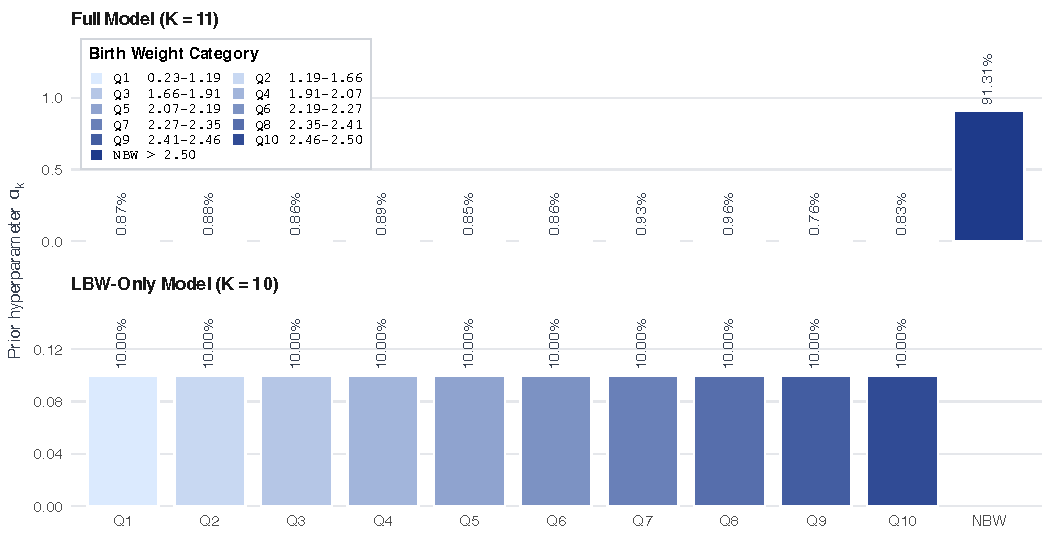
\includegraphics[width=\textwidth]{../../results/2023-2024/article/informed_prior_2023.pdf}
  \caption[Informed Dirichlet priors from 2023 quantiles]{%
    \textbf{Informed Dirichlet prior hyperparameters.} Bar labels give each
    category's share of the total prior mass and the legend gives each
    category's birth-weight interval in kg, both derived from the 2023
    LBW distribution. The full model (top) places 91.3\% of its
    prior mass on the NBW category, so the ten LBW deciles are
    compressed on a linear axis and are read from their labels; the LBW-only
    model (bottom) has no NBW category, hence the empty slot. Panels use
    independent $y$ scales.}
  \label{fig:prior}
\end{figure}
 

\subsection{Notation}
Let \(\mathbf{X}\in\prod_{j=1}^{7}\mathcal{L}_j\) be the fixed \(I \times 7\) predictor matrix, where  \(|\mathcal{L}_j|=(2,3,2,2,2,2,7)\), whose \(i\)th row \(\mathbf{x}_i\) is one class profile. Let \(\mathbf{Y} = [n_{i,k}]_{i=1,\dots,I}^{k=1,\dots,K}\) be the corresponding \(I \times K\) response matrix, so \(\mathbf{y}_i = (n_{i,1}, n_{i,2}, \dots, n_{i,K})\) collects the birth counts of class \(i\) across categories \(k=1,\dots,K\), and \(N_i = \sum_{k=1}^{K} n_{i,k}\) is its total. Each pair \(\mathbf{x}_i, \mathbf{y}_i\) thus records how many births of a given profile fell into each birth-weight category, governed by an unknown probability vector \(\boldsymbol{\theta}_i = (\theta_{i,1}, \dots, \theta_{i,K})\).


% =============================================================================
\section{Methodology}
\label{sec:methods}

\subsection{The Dirichlet-multinomial model}
Within a class, category counts are multinomial given \(\boldsymbol{\theta}_i\) and a conjugate Dirichlet prior is placed on \(\boldsymbol{\theta}_i\):
\begin{align*}
\mathbf{y}_i \mid \mathbf{x}_i
   &\sim \text{Multinomial}^{\ast}(N_i,\boldsymbol{\theta}_i)\\
\boldsymbol{\theta}_i &\sim \mathrm{Dir}(\boldsymbol{\alpha})\\
\boldsymbol{\theta}_i \mid \mathbf{y}_i,\mathbf{x}_i
   &\sim \mathrm{Dir}(\boldsymbol{\alpha}+\mathbf{y}_i).
\end{align*}
The asterisk denotes the omission of the multinomial coefficient since it does not depend on the parameters of interest and retaining it would bias the splitting criterion toward classes with larger total counts. The hyperparameter \(\boldsymbol{\alpha} = (\alpha_1, \dots, \alpha_K)\), with total mass \(\alpha_0 = \sum_{k=1}^{K} \alpha_k\), is set from the previous year's category proportions, which gives an informative, non-degenerate prior for categories that may be empty in any given class. This is one instance of the general advantage of a Bayesian formulation: the prior is the channel through which information external to the current sample --- here, the previous year's national birth-weight distribution --- enters the model, and it does so in a way that is explicit and inspectable rather than implicit in a tuning choice. We suppress the class index \(i\) below, as the derivation is identical for each class profile.

Writing the Dirichlet density and outcome model,
\begin{align*}
  p(\boldsymbol{\theta}\mid\boldsymbol{\alpha})
    &= \frac{\Gamma(\alpha_0)}{\prod_{k}\Gamma(\alpha_k)}
       \prod_{k=1}^{K}\theta_k^{\alpha_k-1},\\
    p(\mathbf{y}\mid\boldsymbol{\theta}, \mathbf{x})
      &\propto \prod_{k=1}^{K}\theta_k^{n_k}
\end{align*}
their product is Dirichlet in \(\boldsymbol{\theta}\) which exhibits conjugacy directly:
\begin{align*}
  p(\mathbf{y},\boldsymbol{\theta}\mid\mathbf{x})
    &\propto \prod_{k=1}^{K}\theta_k^{\,n_k+\alpha_k-1}
     \sim \mathrm{Dir}(\boldsymbol{\alpha}+\mathbf{y}).
\end{align*}
Integrating out \(\boldsymbol{\theta}\) gives the marginal likelihood in closed form,
\begin{align*}
  p(\mathbf{y}\mid\mathbf{x})
    &= \int p(\mathbf{y},\boldsymbol{\theta}\mid\mathbf{x})\,
       d\boldsymbol{\theta}\\
     &= \frac{\Gamma(\alpha_0)}{\Gamma(N+\alpha_0)}
       \prod_{k=1}^{K}\frac{\Gamma(n_k+\alpha_k)}{\Gamma(\alpha_k)}
\end{align*}
and hence, on the log scale,
\begin{equation}
\label{eq:loglik}
\begin{split}
  \ell(\mathbf{y}\mid\mathbf{x})
    =& \log\Gamma(\alpha_0)-\log\Gamma(N+\alpha_0)
       +\sum_{k=1}^{K}\bigl[\log\Gamma(n_k+\alpha_k)-\log\Gamma(\alpha_k)\bigr].
\end{split}
\end{equation}
It is worth being precise about how the prior acts on an empty category. If \(n_k = 0\) then \(\log\Gamma(n_k+\alpha_k) - \log\Gamma(\alpha_k) = 0\), so that category contributes nothing to~\eqref{eq:loglik} and the prior does \emph{not} enter the split criterion through it. The prior's influence on splitting is carried entirely by the normalizing term \(\log\Gamma(\alpha_0) - \log\Gamma(N+\alpha_0)\), which penalizes nodes holding few births and so discourages splits that isolate them. The prior does act directly on empty categories in the posterior mean of the category probabilities, \((n_{i,k}+\alpha_k)/(N_i+\alpha_0)\), which is strictly positive even when \(n_{i,k}=0\). That is what keeps thinly populated classes from being assigned zero probability in a category simply because none was observed.



Because the \(\boldsymbol{\theta}_i\) are independent across classes given \(\boldsymbol{\alpha}\), the full marginal likelihood factorizes as:
\[
  p(\mathbf{Y}\mid\boldsymbol{\alpha},\mathbf{X})
    = \prod_{i=1}^{I}p(\mathbf{y}_i\mid\boldsymbol{\alpha},\mathbf{x}_i),
\]
so on the log scale it is a sum of terms of the form~\eqref{eq:loglik}. This factorization is what makes the criterion practical inside a recursive partitioning algorithm: evaluating a candidate split requires summing~\eqref{eq:loglik} over the two classes routed to the node in question, never over all \(I\).



\subsection{Growing the tree}
Trees are grown with the CART algorithm \cite{breiman1984}, implemented through a custom split rule in the R package \texttt{rpart} \cite{rpart_docs}. A candidate split of node \(t\) into children \(t_L\) and \(t_R\) is scored by the gain in marginal log-likelihood:
\[\Delta\ell = \ell(t_L) + \ell(t_R) - \ell(t)\]
with \(\ell(\cdot)\) the sum of~\eqref{eq:loglik} over the classes routed to that node. The split maximizing \(\Delta\ell\) is taken and the process recurses until a minimum node size or a maximum depth is reached. Trees are grown to a fixed maximum depth rather than pruned because the informed prior already penalizes splits that isolate few births, so the complexity parameter is set to zero and no cross-validated pruning step is used. Replacing an impurity measure with a likelihood is what carries the prior into the splitting decision. A candidate split that isolates a small number of births is not rewarded for the spurious extreme category proportions it produces, because those proportions are shrunk toward \(\boldsymbol{\alpha}\) before being scored. 


\subsection{Categorical splits}
A \(k\)-level unordered predictor admits \(2^{k-1}-1\) possible bipartitions of its levels, but the conventional strategy only evaluates the \(k-1\) splits that are contiguous in some fixed ordering of those levels. For binary predictors that distinction is vacuous: there is a single bipartition and it is contiguous in any ordering, which is why the point is rarely remarked on. At three levels it already bites, if mildly---there are three bipartitions and a contiguous search reaches two of them, whichever two the declared level order happens to make prefixes. For maternal race at seven levels the gap is wide: a contiguous search examines \(6\) of the \(63\) available groupings, and which six depends on nothing more than the order in which the levels are declared. We therefore evaluate all \(2^{k-1}-1\) bipartitions under the same \(\Delta\ell\) criterion and select the maximizer. The cost is negligible because the number of levels is small, and the benefit is that the seven-group encoding of race is real rather than nominal.






\subsection{Uncertainty via a two-tier parametric bootstrap}
\label{sec:methods-boot}

Uncertainty is propagated through an ensemble of \(B=10,000\) trees. Each replicate is generated in two tiers, matching the two ways in which the observed counts table is subject to sampling variation. The first tier redraws how the \(T\) total births are distributed across the \(I\) classes, \(\mathbf{n}^\ast \sim \text{Multinomial}(T, \mathbf{p})\) with \(p_i\) the observed share of the \(T\) births falling in class \(i\), computed once from the observed table and held fixed across replicates; the second redraws, within each class, how its \(n_i^\ast\) births distribute across the categories, using the posterior mean
\[
    \hat{\pi}_{i,k} = \frac{n_{i,k} + \alpha_k}{N_i + \alpha_0}
\]
held fixed across replicates. A tree is fitted to each resampled counts table. Every quantity reported below---category probabilities, aggregate LBW risk, and variable importance---is summarized over the ensemble by its mean and its 95\% percentile interval.

In order to read off the extreme classes (highest- or lowest-risk) from the ensemble, a convention is required. A tree assigns a single posterior to each terminal node, so every class routed to the same node receives an identical mean estimate and percentile interval. The estimate is a property of the node, not of the class, and \emph{the highest- and lowest-risk classes} are therefore sets rather than single classes.
We therefore fix a tolerance and a tie-break. Classes whose posterior mean lies within \(5\%\) of the width of the extremum's percentile interval are treated as indistinguishable, and from that set we report the class with the largest sample size. This tie-break is based on support rather than on the width of the interval, which could be influenced by Monte Carlo variation instead. Naively taking the argmax would order classes on noise, and would systematically favor the thinnest cells, whose intervals are the widest. Two consequences carry into Section~\ref{sec:results-risk} are that the class reported as most extreme need not be the argmax, and in the LBW-only model it is not, and the stability percentages quoted there are measured against the same tolerance, so they report how often the named class is among the indistinguishable extremes of a replicate, not how often it wins a tie-break.


\subsection{Software, reproducibility, and use of AI tools}
\label{sec:methods-software}

All analyses were carried out in R. Trees are fitted with a user-written
splitting method supplied to \texttt{rpart}. The pipeline runs in four stages
(prior-year cutpoints, class-level counts, model fitting with the bootstrap
ensemble, and figure and table generation), driven by modular scripts that read and write intermediate results to disk. Every number, figure, and table in this paper is produced by the analysis code from the source data, and the scripts are organized so that a single command reproduces all results. The code and the derived count tables are available as described in the Data Availability Statement.

During the preparation of this work, the author (Kurth) used Claude (Anthropic) to assist with the software implementation. Specifically, the tool was used to debug and diagnose issues in the R code, and to create custom plotting functions. Since the custom \texttt{rpart} objects are not supported by the package's built-in plotting functions (\texttt{rpart.plot} and \texttt{rpart.plot::prp}), the AI tool was used to generate a custom labeling function for the fitted trees. The author carefully reviewed and takes full responsibility for all code and results. 
The author conceived the study design, selected the predictors and outcomes, specified the model and prior, designed the bootstrap ensemble, and executed the recursive partitioning algorithm. All statistical choices, numerical results, and interpretations are entirely the author's. Furthermore, the initial draft of the manuscript was written exclusively by the author, with AI assistance strictly limited to the coding tasks described above.

\section{Results}
\label{sec:results}

\subsection{Preprocessing and the informed prior}

Of the 3,638,436 live births recorded in 2024, 3,476,907 (95.6\%) are retained after removing records with missing outcomes or a missing predictor. Table~\ref{tab:vars} gives the per-field counts. These are distributed across the \(I\) predictor classes, of which 18 contain no births and are carried by the prior alone. In the 2023 reference year, 8.7\% of births fell below 2.5~kg, so the informed prior assigns \(\alpha_{11} = 0.913\) to the NBW category and divides the remaining 0.087 among the ten LBW deciles, giving the prior mass shown in Figure~\ref{fig:prior}. The deciles are not exactly equal, ranging from 0.76\% to 0.96\% of the total prior mass, because birth weight is recorded in whole grams and cannot be partitioned into exact tenths.



\subsection{Fitted trees}
\label{sec:results-trees}

Both models select maternal race at the root (Figure~\ref{fig:model-trees}), consistent with the documented disparity in LBW incidence across racial groups \cite{marchofdimes2024,kff_maternal_infant_health,pmc1751798}. The full model separates Black mothers from all other groups and grows to 23 terminal nodes; the LBW-only model separates $\{\text{Black},\text{NHOPI}\}$ from the remainder and stops at 8.

% ---- FITTED TREES -- now half a page ---------------------------------------
\begin{figure}[!tp]
  \centering
  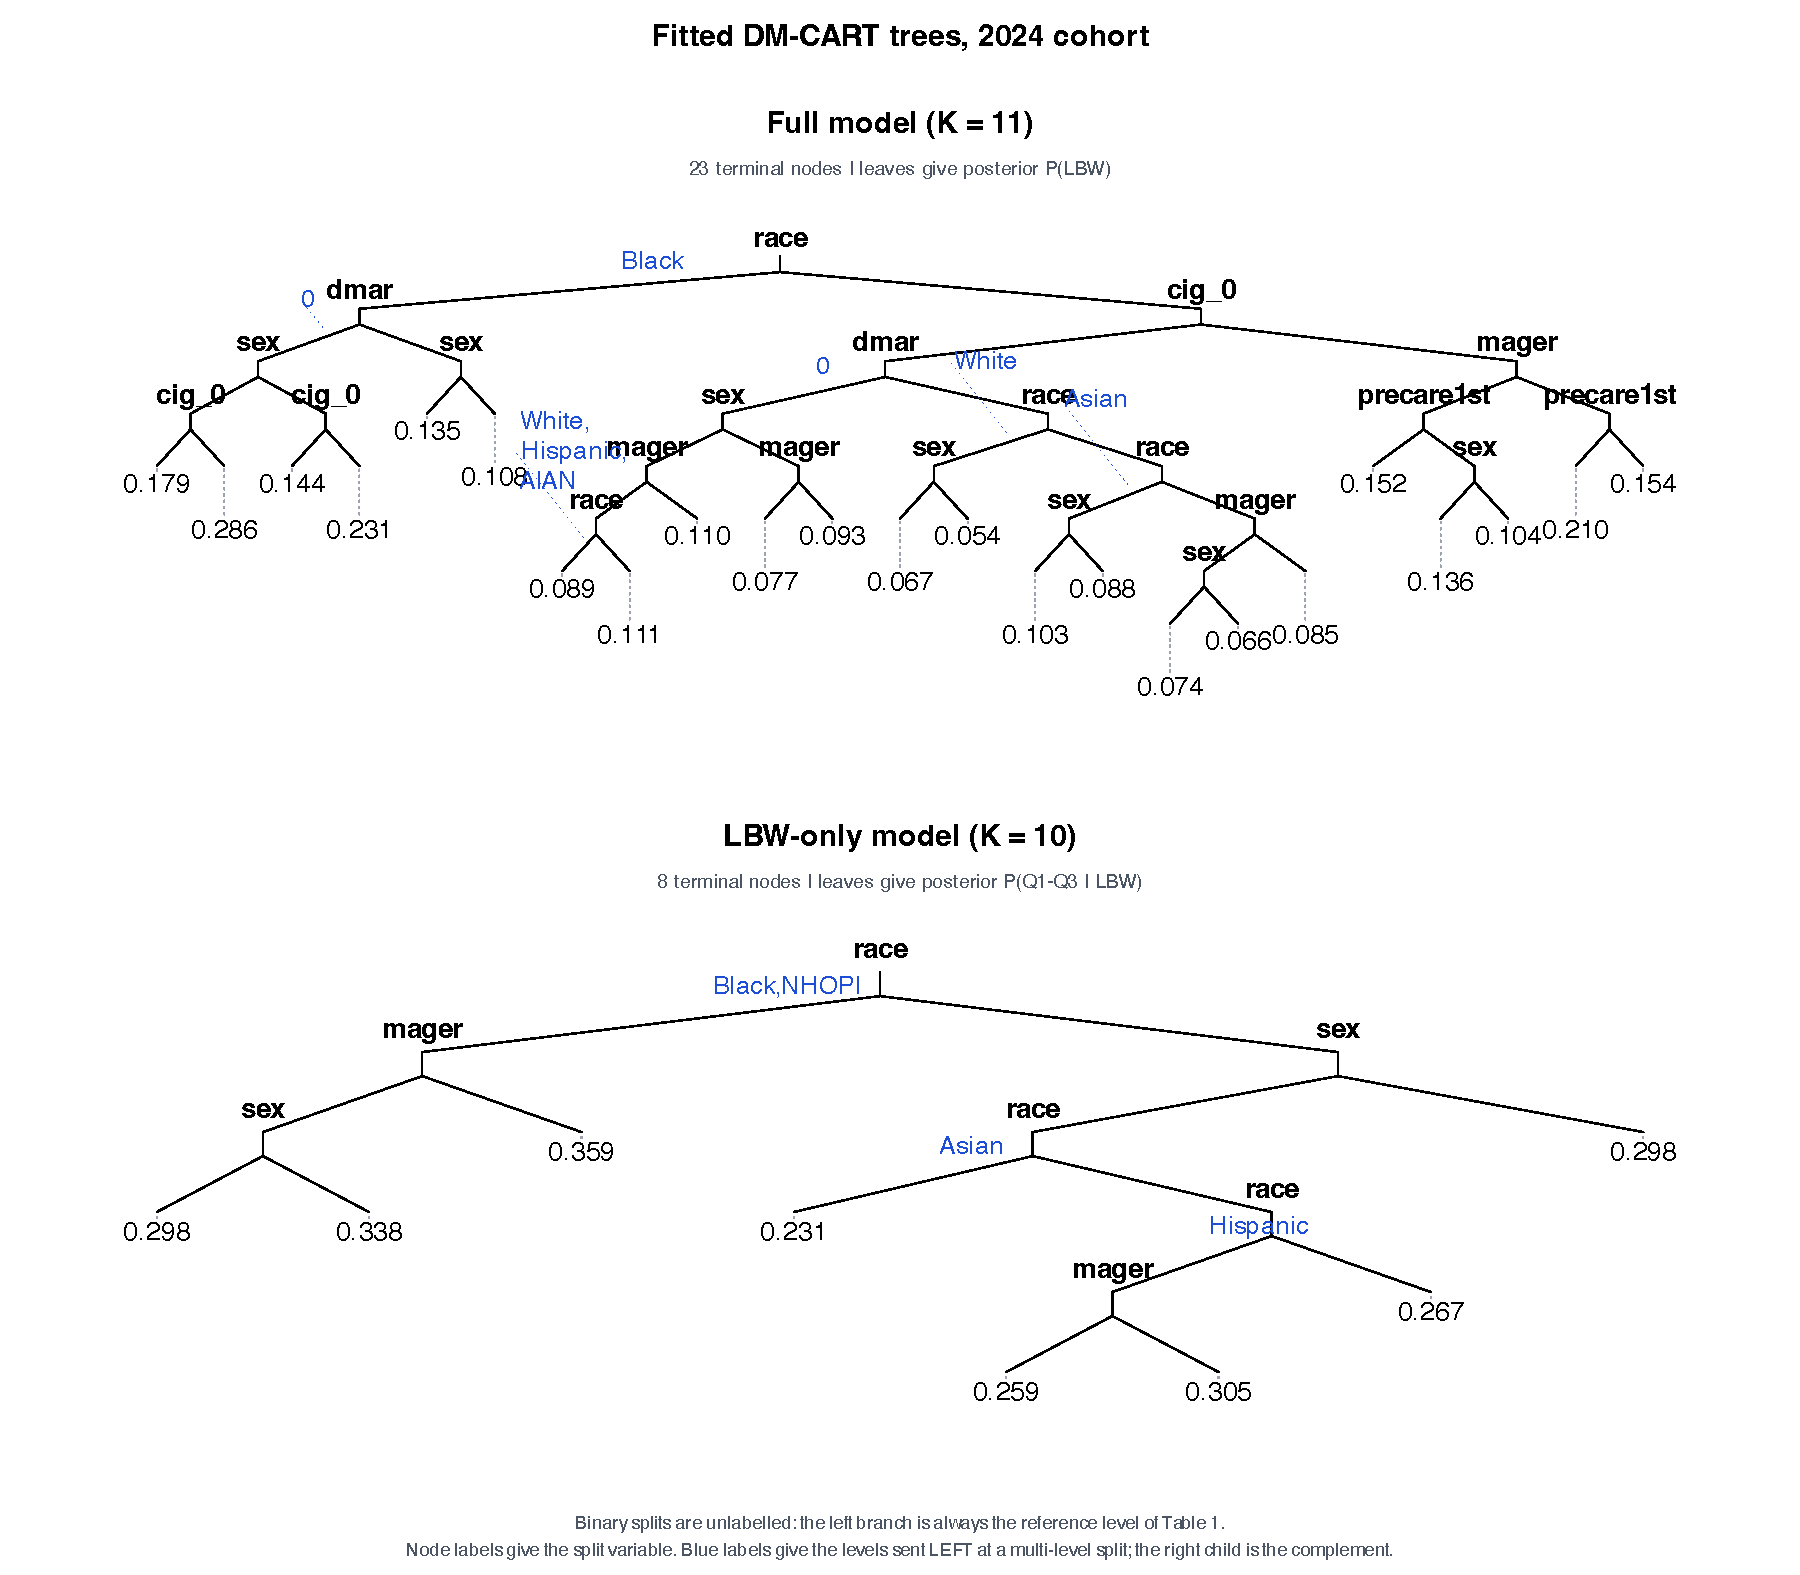
\includegraphics[width=\textwidth]{../../results/2023-2024/article/model_trees_2024.pdf}
  \caption[Fitted DM-CART trees for both model arms]{
    Fitted DM-CART trees for the 2024 cohort: the full model above, the LBW-only
    model below. Node labels give the split variable. Blue labels give the levels
    sent to the left child at a multi-level split, the right child being the
    complement. Binary splits are unlabeled: the left branch is always the
    reference level ($0$) and the right branch the indicator level ($1$) of
    Table~\ref{tab:vars}; \emph{Age} is maternal age over 33, \emph{Education}
    high school completed, \emph{Prenatal} care begun in the first trimester,
    and \emph{Smoking} any pre-pregnancy smoking. Where a label would overlap
    the tree it is drawn clear of it and joined to its branch by a dotted
    leader. Terminal nodes give the number of births and the
    posterior risk of the classes routed there ---
    $P(\mathrm{LBW})$ for the full model and
    $P(Q_1, Q_2 \text{ or } Q_3 \mid \mathrm{LBW})$ for the LBW-only model, in which every
    category is by construction an LBW category, so the two panels are on
    different scales. Both trees select maternal race at the root. Leaf values are read from this tree, not from the ensemble, so they differ slightly from the ensemble means reported in Section~\ref{sec:results-risk}: class 181 has $P(\mathrm{LBW}) = 0.286$ here against an ensemble mean of $0.284$.}
  \label{fig:model-trees}
\end{figure}

The two arms then sharply diverge, and this divergence is the central result. In the full model the branch for Black mothers splits next on marital status and the branch for all other mothers on smoking, with maternal age, prenatal-care timing, and infant sex entering below (see Figure~\ref{fig:model-trees} after root split). In the LBW-only model marital status, smoking, education, and prenatal care are entirely absent from the fitted tree. It splits instead on race again, then infant sex, and maternal age only. Restricting to births already below 2.5~kg removes the contrast that behavioral and socioeconomic factors provide, leaving heterogeneity that biologically-driven factors can explain. This reproduces the qualitative finding of an earlier binary-race analysis of the 2020--2021 cohort \cite{kurth-thesis2025}, in which smoking and marital status ``never'' appeared in the LBW-only tree. The ensemble in Section~\ref{sec:results-ensemble} puts a number on that statement.


Race is also the predictor for which the exhaustive categorical search matters. Two partitions in the fitted full model cannot be reached by the conventional contiguous search over level codes, including the root split itself since $\{\text{Black}\}$ is not a prefix of the declared level order, and one node divides the seven groups as $\{$White, Hispanic, AIAN$\}$ against $\{$Asian, NHOPI, multiracial$\}$, a grouping of several levels on both sides rather than a single level against the rest. Under a binary race contrast none of this structure would be observable.

\subsection{Variable selection across the ensemble}
\label{sec:results-ensemble}

Table~\ref{tab:varfreq} reports how often each predictor is selected across the bootstrap ensemble. Race is the root split in \emph{every} replicate of both models. In the full model, five predictors appear in all replicates, prenatal care in 97.8\%, and maternal education in 53.5\%. The median tree uses all seven predictors across 26.9 splits. The LBW-only model is far sparser, with infant sex, maternal age, and race appearing in every replicate, but prenatal care, marital status, smoking, and education appearing in only 7.3\%, 3.7\%, 2.2\%, and 1.1\% respectively, and the median tree uses three predictors across 7.1 splits.

% Auto-generated by visual.R -- do not edit by hand.
\begin{table}[!htbp]
\centering\small
\caption[Variable importance in the full and LBW-only models]{Variable importance across the 10,000-tree bootstrap ensemble. \emph{Initial split} is the percentage of replicates in which the predictor is chosen at the root; \emph{frequency} the percentage in which it appears anywhere in the tree; \emph{mean depth} its average split depth, with the root at zero. A dash marks a predictor that is never selected.\label{tab:varfreq}}
\begin{tabular*}{\textwidth}{@{\extracolsep\fill}lcc@{}}
\toprule
 & Full model & LBW-only model \\
\cmidrule(lr){2-2} \cmidrule(lr){3-3}
\multicolumn{3}{@{}l}{\textit{Initial split variable}} \\
\midrule
\quad \texttt{race} & 100.0\% & 100.0\% \\
\midrule
\multicolumn{3}{@{}l}{\textit{Variable frequency}} \\
\midrule
\quad \texttt{sex} & 100.0\% & 100.0\% \\
\quad \texttt{dmar} & 100.0\% & 3.7\% \\
\quad \texttt{race} & 100.0\% & 100.0\% \\
\quad \texttt{mager} & 100.0\% & 100.0\% \\
\quad \texttt{precare1st} & 97.8\% & 7.3\% \\
\quad \texttt{cig\_0} & 100.0\% & 2.2\% \\
\quad \texttt{meduc} & 53.5\% & 1.1\% \\
\midrule
\multicolumn{3}{@{}l}{\textit{Mean split depth}} \\
\midrule
\quad \texttt{sex} & 3.72 & 1.44 \\
\quad \texttt{dmar} & 2.84 & 4.43 \\
\quad \texttt{race} & 3.36 & 1.72 \\
\quad \texttt{mager} & 4.11 & 2.14 \\
\quad \texttt{precare1st} & 3.57 & 3.94 \\
\quad \texttt{cig\_0} & 2.40 & 4.10 \\
\quad \texttt{meduc} & 6.40 & 6.04 \\
\midrule
\quad Median predictors per tree & 7 & 3 \\
\quad Mean splits per tree & 26.9 & 7.1 \\
\bottomrule
\end{tabular*}
\end{table}
     % tab:varfreq


Mean split depth separates the predictors further. In the full model smoking (2.40) and marital status (2.84) act early, while education acts late (6.40). Refitting under a depth constraint shows the same ordering from the other direction: the tree grows from 4 terminal nodes and three predictors at depth~2 to 19 nodes and six predictors at depth~5, and maternal education never appears at any depth. Education is therefore not merely the weakest predictor; under a depth constraint it is not used at all.


\subsection{Risk stratification}
\label{sec:results-risk}

Ranking all 672 classes by posterior risk (Figure~\ref{fig:risk-landscape}) produces a smooth gradient rather than a small number of separable strata. Of the 672 classes, 191 meet the support threshold of having at least 1,000 observed births in the full model and 65 in the LBW-only model. The same threshold applies to both models, and the difference in number of qualifying classes reflects the smaller, restricted LBW-only sample. Classes below the support threshold are plotted but excluded from the ranking, because a class with few births contributes almost nothing to its terminal node and its estimate is dominated by its neighboring classes and the prior.

% ---- RISK LANDSCAPE -- single column, stacked -------------------------------
\begin{figure}[!htbp]
  \centering
  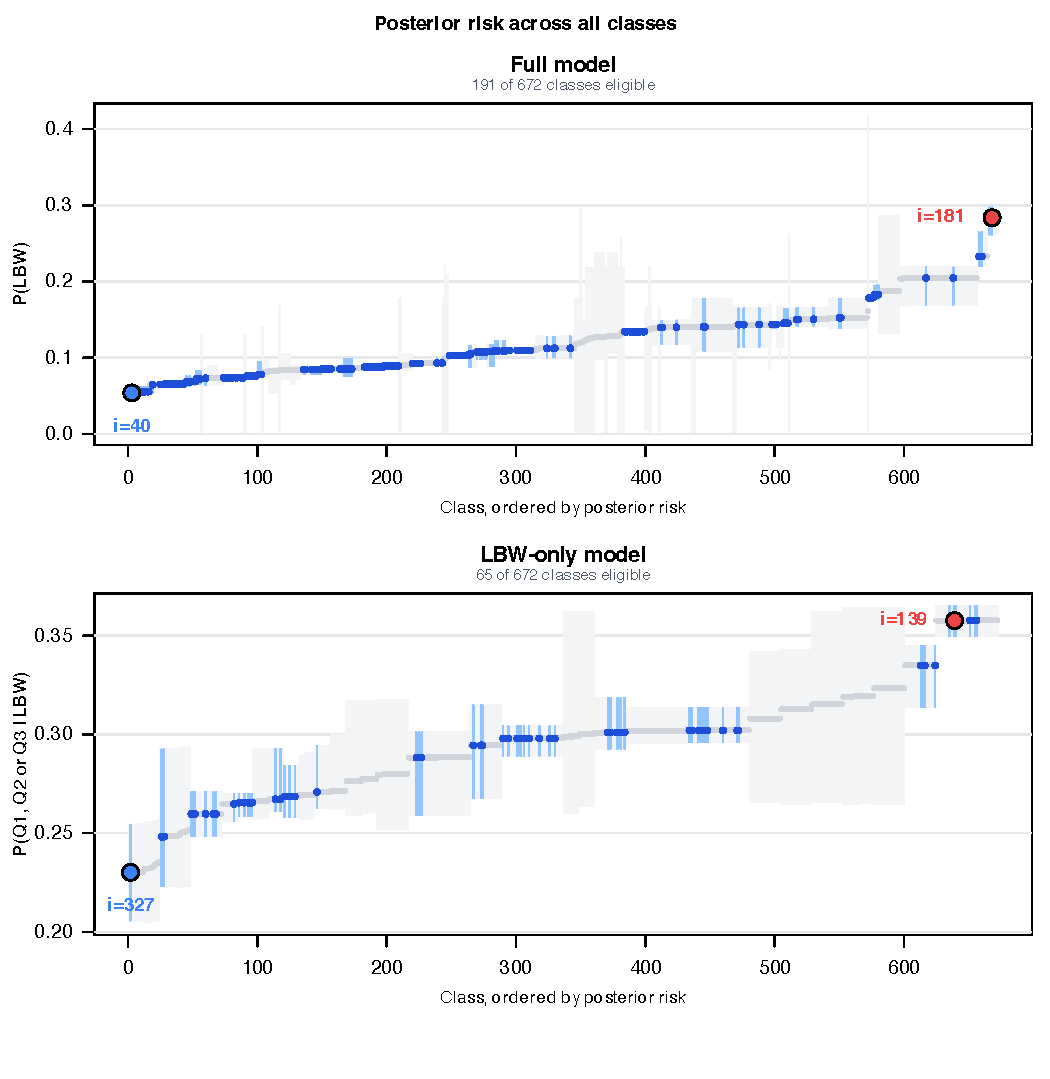
\includegraphics[width=\textwidth]{../../results/2023-2024/article/risk_profile_ranking_2024.pdf}
  \caption[Posterior risk across all classes]{%
    Posterior risk for all 672 maternal-infant classes, the full model above and
    the LBW-only model below, ordered by risk with 95\% percentile bootstrap
    intervals. Filled points are classes meeting the support threshold of
    1{,}000 observed births (191 of 672 in the full model, 65 in the LBW-only
    model); hollow gray points fall below it and are excluded from the ranking,
    but are shown so the extent of the filter is visible. Red and blue mark the
    highest- and lowest-risk class in each arm. Note the two arms use different
    risk scores and therefore different $y$ scales.}
  \label{fig:risk-landscape}
\end{figure}


The highest-risk class in the full model ensemble is a female infant born to an unmarried Black mother aged 33 or under who had smoked before pregnancy, with \(\Pr(\mathrm{LBW}) = 0.284\) \([0.262,0.297]\) over \(N=1,710\) births. The lowest-risk class is a male infant born to a \emph{married} White mother aged 33 or under who had no history of smoking, with \(\Pr(\mathrm{LBW}) = 0.054\) \([0.052, 0.055]\) over \(N=346,814\) births --- a 5.3-fold difference in risk between the extremes. Both are the extreme class in 100\% of bootstrap replicates, and in the full model neither extremum is unique: classes 157 and 181 carry the maximum and classes 28, 40 and 42 the minimum, each set routed to a single terminal node and therefore sharing a posterior exactly. Following Section~\ref{sec:methods-boot} we report from each set the class with the most observed births.


Two features of these profiles are worth stating explicitly. First, the highest-risk profile has \emph{completed} high school (\texttt{meduc} $=1$) and \emph{did} begin prenatal care within the first trimester (\texttt{precare1st}$=1$). Maximum risk is reached through race, marital status, and smoking status without requiring low educational attainment or late care, which is consistent with the minor role education plays in Section~\ref{sec:results-ensemble} and qualifies the weight usually given to maternal education \cite{edu_lbw}. Second, a clinically intuitive ``everything adverse'' epidemiological profile carrying the most extreme combination of risk factors is often \emph{assumed} to be the highest-risk class, but that is not what our rankings report. Here in the full model ensemble, it is not a single class but four, one per combination of infant sex and maternal age, and they rank 1st, 5th, 9th and 13th of 672 with \(N=186\), \(481\), \(161\) and \(509\) births. \emph{Every one of them falls below the support threshold.} The class we do report as highest-risk, class 181, is routed to the same terminal node as the younger female variant and therefore carries not a similar estimate but the identical one --- the same posterior mean and the same interval, $0.284$ $[0.262, 0.297]$. What separates the two is support of $1,710$ observations versus $481$. This is exactly the case the tie-break of Section~\ref{sec:methods-boot} exists to settle, and support is the only ground on which it can be settled. The a priori profile is therefore a rare combination whose apparent extremity is not separable, at this sample size, from that of the class actually reported. Deriving the extremes rather than nominating them does not overturn the clinical intuition here so much as locate it: the adverse combination does sit in the highest-risk node, but the class that is reported as the extreme is the one with the most support.

The LBW-only model asks a different question of the same births, and its extremes have to be read on their own scale. Severity there is $\Pr(Q_1 \cup Q_2 \cup Q_3 \mid \mathrm{LBW})$, the probability that an infant already below 2.5~kg falls in the three smallest deciles. Across eligible classes it runs from $0.230$ $[0.206, 0.254]$ to $0.358$ $[0.350, 0.365]$ --- a 1.6-fold spread, against 5.3-fold in the full model, which is a measure of how much more homogeneous the restricted sample is.
Neither extreme is held as firmly as the full model's, and the two fail in different ways. In the lower pane of Figure~\ref{fig:risk-landscape}, the highest severity class is not unique, with six classes within the $5\%$ interval tolerance. Their posterior means span $0.3577$ to $0.3578$, about half a percent of the width of any one of their intervals, so the ensemble cannot order them. Class 139 is the one reported because it has the most observed births of the six ($N=2{,}783$), not the highest mean. At the bottom there is no such ambiguity: class 327 is the unique minimum. Class 139 is among the highest-severity classes in $98.9\%$ of the 10{,}000 replicates, and class 327 is the lowest-severity class in $98.8\%$.

Table~\ref{tab:commonality} reads down the covariate columns of the ten most extreme classes at each end, and distinguishes a shared feature from an artifact of a single predictor-class cell. In the full model, unmarried status is the only feature common to all ten highest-risk classes, while race is Black in 8 of 10 and smoking is present in 6 of 10 \cite{smoking_lbw}. The two exceptions are informative: classes 67 and 68 are unmarried White mothers over 33 who smoked. The low-risk set is more tightly determined, sharing three unanimous features --- male infants, non-smoking, White --- with the direction of the sex effect matching the established difference in mean birth weight between male and female infants \cite{vanvliet2009decreasing}. High risk is therefore reachable by several routes while low risk requires a specific combination, an asymmetry visible only by examining ten profiles rather than one.

The same reading of the LBW-only rows shows the factors reordering. All ten highest-severity classes are Black and the ten lowest are Asian or Hispanic, so race separates the extremes in this arm as it does in the full model. Smoking does not. It is unanimously absent at \emph{both} ends, which is the shared-feature counterpart of its appearing in only 2.2\% of LBW-only replicates: a predictor that takes the same value in every extreme class cannot be distinguishing between them.

% Auto-generated by visual.R -- do not edit by hand.
\begin{table}[tb]
\centering\footnotesize
\caption[Shared features of the extreme-risk classes]{Shared features of the ten highest- and ten lowest-risk classes. Each cell gives the level carried by most of the ten and how many carry it; \textbf{bold} marks a level shared by all ten. Classes with fewer than 1,000 observed births are excluded.}
\label{tab:commonality}
\begin{tabular}{@{}lcc@{}}
\toprule
\textbf{Predictor} & \textbf{Highest 10} & \textbf{Lowest 10} \\
\midrule
\multicolumn{3}{@{}l@{}}{\textit{Full model}} \\
\quad \texttt{sex} & 0 (7/10) & \textbf{1} (10/10) \\
\quad \texttt{dmar} & \textbf{0} (10/10) & 1 (6/10) \\
\quad \texttt{mager} & 1 (6/10) & 0 (6/10) \\
\quad \texttt{meduc} & 1 (8/10) & 1 (7/10) \\
\quad \texttt{precare1st} & 0 (6/10) & 1 (6/10) \\
\quad \texttt{cig\_0} & 1 (6/10) & \textbf{0} (10/10) \\
\quad \texttt{race} & Black (8/10) & \textbf{White} (10/10) \\
\addlinespace
\multicolumn{3}{@{}l@{}}{\textit{LBW-only model}} \\
\quad \texttt{sex} & 1 (7/10) & \textbf{0} (10/10) \\
\quad \texttt{dmar} & 0 (7/10) & 0 (4/10) \\
\quad \texttt{mager} & 1 (6/10) & 0 (8/10) \\
\quad \texttt{meduc} & 1 (9/10) & 1 (8/10) \\
\quad \texttt{precare1st} & 1 (6/10) & 1 (7/10) \\
\quad \texttt{cig\_0} & \textbf{0} (10/10) & \textbf{0} (10/10) \\
\quad \texttt{race} & \textbf{Black} (10/10) & Hispanic (7/10) \\
\bottomrule
\end{tabular}
\end{table}
 % tab:commonality

Figure~\ref{fig:risk-profile} gives the category probability estimate profiles behind both pairs of extremes (classes 181 and 40 for full model, classes 139 and 327 for LBW-only), and the two models behave differently in a way their aggregate risks conceal. In the full model the two profiles are close to flat and differ almost entirely in magnitude, with class 181 carrying between $0.019$ and $0.033$ versus class 40's $0.005$ to $0.006$ in each LBW decile, and neither tilts appreciably toward the smallest weights. What separates the two is how much mass sits below 2.5~kg at all, not how it is arranged once it is there. In the LBW-only model the two profiles slope in opposite directions, with class 139 falling from $0.134$ in $Q_1$ to $0.079$ in $Q_{10}$ while class 327 rises from $0.071$ to a peak of $0.128$ in $Q_8$. The same total mass is distributed in opposite directions, which is the severity gradient a binary indicator collapses and which is visible only because the outcome was retained as a distribution.


% ---- CATEGORY PROBABILITIES FOR THE EXTREME CLASSES -------------------------
\begin{figure}[!tp]
  \centering
  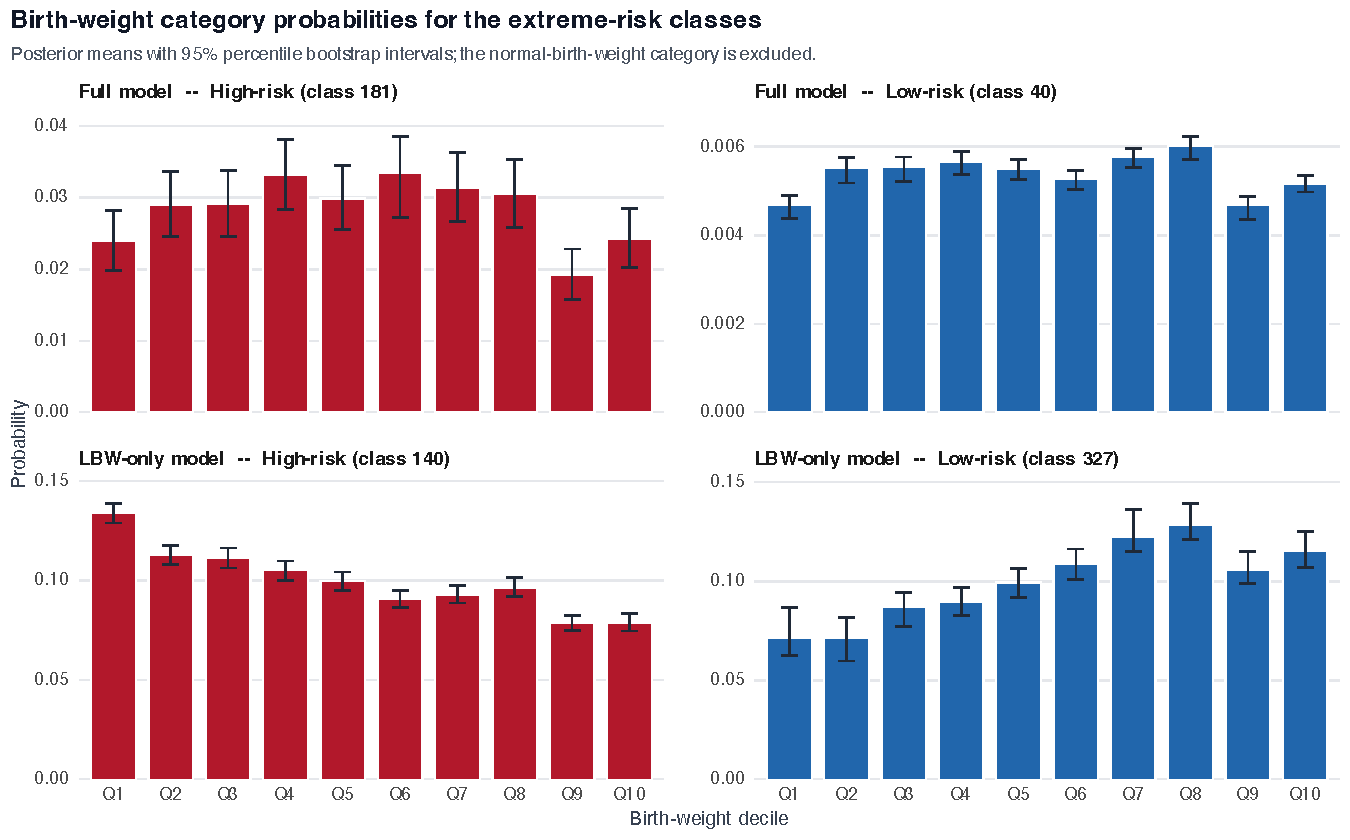
\includegraphics[width=0.94\textwidth]{../../results/2023-2024/article/risk_category_profiles_2024.pdf}
  \caption[Category probabilities for the extreme-risk classes]{%
    Posterior probability of each low-birth-weight decile for the highest- and
    lowest-risk class of each model arm, with 95\% percentile bootstrap intervals
    from the 10{,}000-tree ensemble. The normal-birth-weight category is excluded
    so the shape within the LBW region is visible; panels use independent $y$
    scales. Note the full-model panels are close to flat while the LBW-only
    panels slope in opposite directions; the body text reads this off.}
  \label{fig:risk-profile}
\end{figure}


\section{Discussion and Conclusion}
\label{sec:conclusion}

This study applies recursive partitioning, driven by a Dirichlet-Multinomial likelihood, to the full discretized birth-weight distribution rather than to a binary threshold indicator. The conjugate prior supplies the closed-form splitting criterion and, more importantly, stabilizes the sparse cells that a finely-resolved predictor space produces. That stabilization is what makes this substantive contribution possible: maternal race enters at the full seven-level resolution, and marital status retains the explicit \emph{unknown} level rather than discarding the 11.1\% of records for which it is not reported.

Three findings follow.
First, the determinants of \emph{crossing} the LBW threshold and the determinants of \emph{severity given} LBW are different sets of variables. Marital status, smoking, education and prenatal care are selected in essentially every full-model replicate and in almost no LBW-only replicate (3.7\%, 2.2\%, 1.1\% and 7.3\%). Behavioral and socioeconomic factors govern whether an infant falls below 2.5~kg; among those who do, race, infant sex, and maternal age govern how far below. A binary LBW outcome cannot express this distinction, because it collapses the second question entirely.

This result runs against a reasonable prior expectation and should be read carefully, that social determinants should shape how small a LBW infant is, not merely whether the threshold is crossed---and it should be read carefully. Absence of selection is not absence of effect. Restricting to births below 2.5~kg removes roughly 91\% of the sample and, with it, most of the contrast these variables explain: what remains is a comparatively homogeneous group in which a greedy criterion finds little further deviance to remove. The ensemble does not license the statement that smoking or marital status is unrelated to severity, only that neither improves the partition once the outcome is restricted. Race is the informative exception: it survives the restriction and is selected at the root of both models, which is precisely the pattern one would expect of a factor operating on the whole distribution rather than at the threshold alone.

Second, derived risk profiles differ from assumed ones in ways that matter for targeting. The empirical highest-risk class has completed high school and received first-trimester care, while the ``everything adverse'' profile that one would assume \emph{a priori} to carry the highest risk splits into four variants ranking between 1st and 13th, none of which clears the support threshold. An analysis that fixes the comparison groups in advance would have reported the rare profile as the high-risk group and would have attributed to education and prenatal care a role the ensemble does not support. Reading ten extreme profiles rather than one also shows that high risk is reachable by several routes, whereas low risk requires a specific combination.


Third, resolution in a categorical predictor is itself a finding. Race is the root split in 100\% of replicates in both models, and the fitted partitions include groupings, such as $\{$White, Hispanic, AIAN$\}$ against $\{$Asian, NHOPI, multiracial$\}$, that a binary contrast cannot express by construction and that a conventional contiguous search over level codes could not reach. The combination of the informed Dirichlet prior and the exhaustive search over bipartitions is what makes this resolution admissible: thin groups keep honest, wide intervals rather than being collapsed away or reported with false precision.

\bmsubsection*{Limitations}

Several constraints qualify these results. Marital status is missing for 11.1\% of records, and because the public-use file suppresses every geographic identifier the mechanism generating that missingness cannot be modeled. We therefore carry \emph{unknown} as a level rather than imputing these values, and the fitted trees group it with the married category, which is a finding about reporting areas rather than about mothers. The support threshold of 1{,}000 births is a judgment, not a derived quantity. A different threshold would admit different extreme classes, which is why Figure~\ref{fig:risk-landscape} shows the excluded classes rather than hiding them. The shared-feature analysis in Table~\ref{tab:commonality} depends on the size of the extreme set --- ten was chosen to be large enough to distinguish a pattern from a single cell and small enough to remain extreme --- and a different cut-off would change which features reach unanimity, so it should be read as descriptive rather than inferential. \texttt{precare1st} records when prenatal care began, not its adequacy in the Kotelchuck sense, which is not available in this analysis. The predictor set is small by design, and enlarging it is the obvious extension. Because classes are the cross-classification of the predictors, each additional field multiplies the class space and hence the cost of every likelihood evaluation, so a richer model would need either coarser encodings or a search that does not enumerate all classes. Finally, the design is observational and the classes are defined by covariate combination, so the reported quantities are risks conditional on a profile, not causal effects of any component of it.

\bmsubsection*{Conclusion}

Modeling the full discretized birth-weight distribution with a Dirichlet-Multinomial tree preserves the severity information a binary threshold discards, and quantifies risk at the resolution of a complete covariate profile with an interval attached. Applied to the 2024 U.S. Natality dataset, it separates the determinants of crossing the LBW threshold from the determinants of severity below it, identifies extreme-risk profiles that a covariate-reading approach would not have nominated, and supports a seven-level treatment of maternal race that a plain multinomial tree could not. The same framework applies to any setting where an ordered categorical outcome is routinely dichotomized and where the interesting subgroups are thin.



% =============================================================================
%  BACK MATTER
%  USG.cls provides \bmsection*{} / \bmsubsection*{} for unnumbered back-matter
%  headings; plain \section*{} is not styled by the class.
% =============================================================================

\bmsection*{Acknowledgments}
The author (Kurth) thanks Professor Christopher H. Schmid (Brown University) for comments on an earlier version of this work.

\bmsection*{Author Contributions}
% CRediT taxonomy.
\textbf{Adam M. Kurth:} conceptualization; methodology; software; formal
analysis; data curation; visualization; writing -- original draft; writing --
\textbf{P. Richard Hahn:} conceptualization; methodology; supervision;
review and editing.
The author (Kurth) read and approved the final manuscript.

\bmsection*{Financial Disclosure}
None reported.

\bmsection*{Conflict of Interest}
The authors declare no potential conflict of interest.

\bmsection*{Data Availability Statement}
% Journal requirement: "Statistics in Medicine expects that data supporting the
% results reported in the paper will be archived in an appropriate public
% repository ... Authors will be able to complete a data accessibility
% statement which will be published with their paper."
The data that support the findings of this study are openly available. The
analysis uses the 2023 and 2024 U.S. Natality public-use micro-data files
published by the National Center for Health Statistics, which are available
without restriction from the NCHS Vital Statistics data portal at
\url{https://www.nber.org/research/data/vital-statistics-natality-birth-data}. The files contain no direct identifiers and all geographic identifiers are suppressed by
NCHS before release, so no ethics approval was required for this secondary
analysis. The derived $672 \times K$ class-by-category count tables that are
the direct input to the models, together with the fitted bootstrap ensembles,
are deposited with the analysis code.

\bmsection*{Code Availability}
The R (version 4.5.0) implementation of the Dirichlet-Multinomial splitting rule, the two-tier parametric bootstrap, and all scripts that reproduce every figure and table in this paper are available at \url{https://github.com/adamkurth/dm-cart} and archived at \url{https://doi.org/10.5281/zenodo.22089989}, which is release \texttt{v1.0.0}, the version used for the results reported here. A single driver shell script regenerates the full set of results from the raw natality files, and the bootstrap is seeded, so a re-run on the same input reproduces the numbers in this paper exactly.

\bibliography{references}

\end{document}
